\documentclass[]{elsarticle} %review=doublespace preprint=single 5p=2 column
%%% Begin My package additions %%%%%%%%%%%%%%%%%%%
\usepackage[hyphens]{url}

  \journal{BioR\(\chi\)iv} % Sets Journal name


\usepackage{lineno} % add

\usepackage{graphicx}
%%%%%%%%%%%%%%%% end my additions to header

\usepackage[T1]{fontenc}
\usepackage{lmodern}
\usepackage{amssymb,amsmath}
\usepackage{ifxetex,ifluatex}
\usepackage{fixltx2e} % provides \textsubscript
% use upquote if available, for straight quotes in verbatim environments
\IfFileExists{upquote.sty}{\usepackage{upquote}}{}
\ifnum 0\ifxetex 1\fi\ifluatex 1\fi=0 % if pdftex
  \usepackage[utf8]{inputenc}
\else % if luatex or xelatex
  \usepackage{fontspec}
  \ifxetex
    \usepackage{xltxtra,xunicode}
  \fi
  \defaultfontfeatures{Mapping=tex-text,Scale=MatchLowercase}
  \newcommand{\euro}{€}
\fi
% use microtype if available
\IfFileExists{microtype.sty}{\usepackage{microtype}}{}
\usepackage[margin=1in]{geometry}
\bibliographystyle{elsarticle-harv}
\ifxetex
  \usepackage[setpagesize=false, % page size defined by xetex
              unicode=false, % unicode breaks when used with xetex
              xetex]{hyperref}
\else
  \usepackage[unicode=true]{hyperref}
\fi
\hypersetup{breaklinks=true,
            bookmarks=true,
            pdfauthor={},
            pdftitle={Measurement error associated with gait cycle selection in treadmill running at various speeds},
            colorlinks=false,
            urlcolor=blue,
            linkcolor=magenta,
            pdfborder={0 0 0}}
\urlstyle{same}  % don't use monospace font for urls

\setcounter{secnumdepth}{0}
% Pandoc toggle for numbering sections (defaults to be off)
\setcounter{secnumdepth}{0}


% tightlist command for lists without linebreak
\providecommand{\tightlist}{%
  \setlength{\itemsep}{0pt}\setlength{\parskip}{0pt}}






\begin{document}


\begin{frontmatter}

  \title{Measurement error associated with gait cycle selection in
treadmill running at various speeds}
    \author[Centre for Sport Research]{Aaron S. Fox\corref{1}}
  
    \author[Centre for Sport Research]{Jason Bonacci}
  
    \author[UNSW]{John Warmenhoven}
  
    \author[Centre for Sport Research]{Meghan F. Keast}
  
      \address[Centre for Sport Research]{Centre for Sport Research,
School of Exercise and Nutrition Sciences, Deakin University, Geelong,
Australia}
    \address[UNSW]{School of Engineering and Information Technology,
University of New South Wales, Canberra, Australia}
      \cortext[1]{Corresponding Author}
  
  \begin{abstract}
  Insert abstract\ldots{}
  \end{abstract}
  
 \end{frontmatter}

\hypertarget{introduction}{%
\section{Introduction}\label{introduction}}

Collecting and analysing running biomechanics is a common method for
understanding relationships between running technique and performance
\textbf{\emph{{[}ADD REFS{]}}} or injury/pain \textbf{\emph{{[}ADD
REFS{]}}}, and evaluating changes in running technique following
training or interventions \textbf{\emph{{[}ADD REFS{]}}}. A common
approach across this form of study is to average data from a certain
number of gait cycles to compute a given biomechanical measure --- and
this is thought to be representative of the individual. Given the
inherent variability in human movement (\textbf{vanEmmerik2000?}), the
number of and how gait cycles are selected to create this
`representative mean' appears an important choice in accurately
quantifying an individuals running gait. However, the number of gait
cycles used in biomechanical studies of running widely varies across the
literature (\textbf{Oliveira2021?}). Further, from our groups experience
reading such studies --- very rarely (if ever) has the decision process
underpinning how many gait cycles are used been specifically explained.

~

We can collect a significant number of gait cycles from runners during
laboratory- or clinic-based testing, particularly if a treadmill is
used. Having participants settle into a steady rhythm via an extended
period of running may be advantageous in producing a more habitual
running pattern \textbf{\emph{{[}REF for this???{]}}}. The use of a
significant number of gait cycles becomes a greater issue when analysing
these data. Inflated data cleaning (e.g.~labelling and gap filling
motion capture data) and analysis (e.g.~processing frames via inverse
kinematics) times will occur when processing a running trial that uses
many versus fewer gait cycles. Similarly, the increased data storage
needs (i.e.~larger file sizes) associated with trials including more
gait cycles could introduce difficulties in certain circumstances. There
is subsequently a need to understand the impact gait cycle selection
processes have on biomechanical measures to help optimise data
collection and analysis practices without adversely impacting the
research outcomes.

~

Oliveira and Pirscoveanu(\textbf{Oliveira2021?}) recently examined the
typical number of gait cycles used in running biomechanics studies. On
average, studies used 12 cycles per runner to describe running
biomechanics, while Very few (5 out of 56 studies examined) used more
than 10 cycles (\textbf{Oliveira2021?}). Oliveira and
Pirscoveanu(\textbf{Oliveira2021?}) subsequently performed a study
investigating the impact of sample size (i.e.~10 to 40 runners) and the
number of gait cycles (i.e.~5 to 40 steps) used on biomechanical
measures --- specifically, foot contact time, loading rate, peak
vertical ground reaction force, peak braking force, running speed, and
foot contact angle. They suggested greater than 10 steps are typically
required to achieve stable biomechanical measures in runners, and
collecting at least 25 steps will increase the likelihood of achieving
stability in the range of biomechanical measures examined across a
cohort of runners (\textbf{Oliveira2021?}). These findings are, however,
specific to overground running and the set of biomechanical measures
analysed. Treadmill running is often used in research
(\textbf{VanHooren2020?}), and it is plausible that treadmill running
may incur a different pattern with respect to the number of gait cycles
needed for analyses. Further, Oliveira and
Pirscoveanu(\textbf{Oliveira2021?}) did not examine lower limb kinematic
variables commonly used in gait biomechanics studies. These kinematic
variables are presented as both `zero-dimensional' (0D; e.g.~peak
values) and `one-dimensional' (1D; e.g.~time-normalised kinematic
waveform) variables across biomechanical studies \textbf{\emph{{[}ADD
REFS{]}}}. Analyses of these common kinematic variables in both their 0D
and 1D forms may yield additional details with respect to the number of
gait cycles required in biomechanical research. Lastly, Oliveira and
Pirscoveanu's(\textbf{Oliveira2021?}) analyses were driven by
understanding data stability and statistical significance between two
running conditions (i.e.~`normal' vs.~`silent' running). A different
approach focused on understanding the magnitude of `error' can further
our understanding of how gait cycle selection practices impact
biomechanical measures. Specifically, understanding the potential
`error' or variability introduced by selecting different number of gait
cycles can aid in interpreting the legitimacy of an effect (i.e.~could
small effects be due to the set of gait cycles selected).

~

We sought to extend our current understanding of how the number of gait
cycles selected for analysis impact lower limb kinematic measures from a
continuous bout of treadmill running. First, we examined the magnitude
of `error' introduced in the representative mean compared to the entire
bout of treadmill running when the number of gait cycle samples is
varied. Second, we examined the potential variation introduced in the
representative mean when sampling a specific number of gait cycles from
different sections of the running bout.

\hypertarget{methods}{%
\section{Methods}\label{methods}}

\hypertarget{dataset}{%
\subsection{Dataset}\label{dataset}}

~

We used the public dataset of treadmill running biomechanics from
Fukuchi et al.(\textbf{Fukuchi2017?}). The specifics of this dataset can
be found in the associated paper (\textbf{Fukuchi2017?}). Briefly, this
dataset contains lower-extremity kinematics and kinetics of 28 regular
runners (27 male, 1 female; age = 34.8 ± 6.7 years; height = 176.0 ± 6.8
cm; mass = 69.6 ± 7.7 kg; running experience = 8.5 ± 7.0 years; running
pace = 4.1 ± 0.4 min/km) (\textbf{Fukuchi2017?}). Running kinematics
were collected using a 12-camera 3D motion capture system (Raptor-4,
Motion Analysis, Santa Rosa, CA, United States) and ground reaction
force (GRF) data via an instrumented dual-belt treadmill (FIT, Bertec,
Columbus, OH, United States) (\textbf{Fukuchi2017?}). Participants ran
on the treadmill at three designated speeds (2.5m·s\textsuperscript{-1},
3.5m·s\textsuperscript{-1} and 4.5m·s\textsuperscript{-1}), during which
a three-minute accommodation period was provided followed by a 30-second
data collection period (\textbf{Fukuchi2017?}).

~

We processed the experimental data from Fukuchi et
al.(\textbf{Fukuchi2017?}) using OpenSim 4.0 (\textbf{Delp2007?}).
Segment geometry of the generic musculoskeletal model of the pelvis and
lower limb provided by Lai et al.(\textbf{Lai2017?}) were scaled for
each participant using their static calibration trial, which was also
used as a reference for adjusting marker positions on the model. Lower
limb joint angles were calculated using filtered (10Hz low-pass
4\textsuperscript{th} order Butterworth) marker trajectory data within
inverse kinematics analysis. GRF data were filtered using the same
cut-off frequency and filter. The filtering procedures reflected those
originally performed by Fukuchi et al.(\textbf{Fukuchi2017?}). Foot
strike and toe-off events were determined when the vertical GRF crossed
a 20N threshold, also in line with the original work
(\textbf{Fukuchi2017?}).

\hypertarget{data-analysis}{%
\subsection{Data Analysis}\label{data-analysis}}

~

Kinematic variables common to gait biomechanics studies (i.e.~hip
flexion/extension, hip adduction/abduction, hip internal/external
rotation, knee flexion and ankle plantarflexion/dorsiflexion) were
extracted from the right limb for all participants. Data between
consecutive foot strikes were extracted and time-normalised to 0-100\%
of the gait cycle. The time-normalised one-dimensional (1D) curves were
used in subsequent 1D analyses, while a set of peak variables (hip
flexion, hip adduction, hip internal rotation, knee flexion, ankle
dorsiflexion) were calculated and extracted for the zero-dimensional
(0D) analyses.

~

To examine how the number of gait cycles used impacts a participants
representative kinematic mean, we determined `ground truth' values to
compare to for the 0D and 1D kinematic variables by calculating the mean
from all available gait cycles in the 30-second bout of treadmill
running. This value was thought to be the `most representative' of each
participants average running kinematics, and was not influenced by the
selection of a subset of gait cycles from the running bout. We then
iteratively calculated mean values across the kinematic variables using
a range (\emph{n} = 5 --- 30) of gait cycles from the treadmill running
bout. For each iteration, a random sample of \emph{n} consecutive gait
cycles were extracted from the treadmill running bout and used to
calculate a representative kinematic mean. We then compared this
representative kinematic mean to the `ground truth' value for the
respective variable to determine the `error' that gait cycle number
selection could introduce. For 0D variables, the absolute difference
between the representative mean and `ground truth' was recorded in each
sampling iteration. For 1D variables, the absolute difference between
the representative mean and `ground truth' at each point across the
time-normalised gait cycle were calculated, and the peak difference
recorded. The random sampling process for each \emph{n} of gait cycles
was repeated 1,000 times for each participant at each running speed ---
and the error values collated to present descriptive statistics
(i.e.~mean ± standard deviation {[}SD{]}, median, range, inter-quartile
range) for each gait cycle number across the kinematic variables and
running speeds.

~

To examine how sampling gait cycles from different sections of the
running bout impacts a participants representative kinematic mean, we
iteratively calculated representative kinematic means using a range
(\emph{n} = 5 --- 15) of randomly sampled consecutive gait cycles from
different sections of the running bout. A smaller range of gait cycles
was required for this analysis to avoid sharing gait cycles between the
calculated means. For each sampling iteration, we randomly sampled
\emph{n} consecutive gait cycles from two sections of the running bout.
We then compared the calculated representative kinematic means between
the two sampled sections to determine the `error' or variation that
selection of gait cycles from different sections of the running bout
could introduce. For 0D variables, the absolute difference between the
two representative means was recorded in each sampling iteration. For 1D
variables, the absolute difference between the two representative means
was calculated at each point across the time-normalised gait cycle, and
the peak difference recorded. The random sampling process for each
\emph{n} of gait cycles was repeated 1,000 times for each participant at
each running speed --- and the error values collated to present
descriptive statistics (i.e.~mean ± standard deviation {[}SD{]}, median,
range, inter-quartile range) for each gait cycle number across the
kinematic variables and running speeds.

\hypertarget{results}{%
\section{Results}\label{results}}

\hypertarget{how-does-the-number-of-gait-cycles-used-impact-the-representative-kinematic-mean}{%
\subsection{How does the number of gait cycles used impact the
representative kinematic
mean?}\label{how-does-the-number-of-gait-cycles-used-impact-the-representative-kinematic-mean}}

~

The mean, variance and range of the absolute error of the representative
kinematic mean (i.e.~compared to the mean from all gait cycles) for the
peak 0D kinematic variables progressively reduced as the number of gait
cycles used increased (see Figures \ref{fig:groundTruthError_runT25_0D},
\ref{fig:groundTruthError_runT35_0D} and
\ref{fig:groundTruthError_runT45_0D}). In particular, increasing the
number of gait cycles used reduced the range of potential error compared
to the `ground truth' mean. Similar magnitudes of `error' were observed
between the 2.5m·s\textsuperscript{-1} and 3.5m·s\textsuperscript{-1}
speeds across the 0D kinematic variables at comparable gait cycle
numbers --- where the maximum errors were less than 1 degree even when
using a small number of gait cycles. This contrasted to the
4.5m·s\textsuperscript{-1} speed where maximum errors typically exceeded
1-2 degrees, particularly for peak hip and knee joint angles when a
lower number of gait cycles were used. Subsequently, a much higher
number of gait cycles (i.e.~25-30) achieved similar magnitudes of error
to fewer gait cycles (i.e.~\textless{} 10) for running at
4.5m·s\textsuperscript{-1} versus the other two speeds, respectively.
The larger `error' values observed at 4.5m·s\textsuperscript{-1}
appeared to be driven by a bimodal distribution of the error --- whereby
certain sampling iterations within the same biomechanical measure could
produce relatively higher versus lower errors (see Figure
\ref{fig:groundTruthError_runT45_0D}). The exception to this difference
at the higher speed was for peak ankle dorsiflexion, where similarly low
`error' values and ranges (i.e.~\textless{} 0.5 degrees) were observed
across all speeds.

~

\begin{figure}

{\centering \includegraphics[width=1\linewidth]{D:/+GitRepos+/biomech-trial-selection/Analysis/GroundTruthComp/Figures/AbsoluteError_NoGaitCycle_runT25_0D} 

}

\caption{Absolute error in peak kinematic variables (i.e. zero-dimensional [0D]) when running at 2.5m·s$^{-1}$ using a subset of gait cycles versus all gait cycles from the 30-second treadmill bout. Darker points and solid lines equate to the mean ± standard deviation. Horizontal lines within boxes equate to the median value, boxes indicate the 25$^{th}$ to 75$^{th}$ percentile, and dashed whiskers indicate the range. Shaded violins are included to illustrate the distribution of values. FLEX — flexion; EXT — extension; ADD — adduction; ABD — abduction; IR — internal rotation; ER — external rotation; DF — dorsiflexion; PF — plantarflexion.}\label{fig:groundTruthError_runT25_0D}
\end{figure}

\begin{figure}

{\centering \includegraphics[width=1\linewidth]{D:/+GitRepos+/biomech-trial-selection/Analysis/GroundTruthComp/Figures/AbsoluteError_NoGaitCycle_runT35_0D} 

}

\caption{Absolute error in peak kinematic variables (i.e. zero-dimensional [0D]) when running at 3.5m·s$^{-1}$ using a subset of gait cycles versus all gait cycles from the 30-second treadmill bout. Darker points and solid lines equate to the mean ± standard deviation. Horizontal lines within boxes equate to the median value, boxes indicate the 25$^{th}$ to 75$^{th}$ percentile, and dashed whiskers indicate the range. Shaded violins are included to illustrate the distribution of values. FLEX — flexion; EXT — extension; ADD — adduction; ABD — abduction; IR — internal rotation; ER — external rotation; DF — dorsiflexion; PF — plantarflexion.}\label{fig:groundTruthError_runT35_0D}
\end{figure}

\begin{figure}

{\centering \includegraphics[width=1\linewidth]{D:/+GitRepos+/biomech-trial-selection/Analysis/GroundTruthComp/Figures/AbsoluteError_NoGaitCycle_runT45_0D} 

}

\caption{Absolute error in peak kinematic variables (i.e. zero-dimensional [0D]) when running at 4.5m·s$^{-1}$ using a subset of gait cycles versus all gait cycles from the 30-second treadmill bout. Darker points and solid lines equate to the mean ± standard deviation. Horizontal lines within boxes equate to the median value, boxes indicate the 25$^{th}$ to 75$^{th}$ percentile, and dashed whiskers indicate the range. Shaded violins are included to illustrate the distribution of values. FLEX — flexion; EXT — extension; ADD — adduction; ABD — abduction; IR — internal rotation; ER — external rotation; DF — dorsiflexion; PF — plantarflexion.}\label{fig:groundTruthError_runT45_0D}
\end{figure}

We observed near identical characteristics of the mean, variance and
range of the peak absolute error of the representative kinematic mean
(i.e.~compared to the mean from all gait cycles) for the 1D kinematic
variables (see Figures \ref{fig:groundTruthError_runT25_1D},
\ref{fig:groundTruthError_runT35_1D} and
\ref{fig:groundTruthError_runT45_1D}). As with the 0D variables, the
potential `error' reduced as the number of gait cycles increased, and
similarly low magnitudes of `error' (i.e.~\textless{} 1 degree) were
observed between the 2.5m·s\textsuperscript{-1} and
3.5m·s\textsuperscript{-1} speeds across the 1D kinematic variables at
comparable gait cycle numbers. Larger `errors' exceeding 1-2 degrees
with lower gait cycle numbers were present at the
4.5m·s\textsuperscript{-1} speed (with the exception of ankle
dorsi/plantarflexion), with this again appearing to be driven by a more
bimodal distribution of samples (see Figure
\ref{fig:groundTruthError_runT45_1D}).

~

\begin{figure}

{\centering \includegraphics[width=1\linewidth]{D:/+GitRepos+/biomech-trial-selection/Analysis/GroundTruthComp/Figures/AbsoluteError_NoGaitCycle_runT25_1D} 

}

\caption{Peak absolute error in kinematic variables across the gait cycle (i.e. one-dimensional [1D]) when running at 2.5m·s$^{-1}$ using a subset of gait cycles versus all gait cycles from the 30-second treadmill bout. Darker points and solid lines equate to the mean ± standard deviation. Horizontal lines within boxes equate to the median value, boxes indicate the 25$^{th}$ to 75$^{th}$ percentile, and dashed whiskers indicate the range. Shaded violins are included to illustrate the distribution of values. FLEX — flexion; EXT — extension; ADD — adduction; ABD — abduction; IR — internal rotation; ER — external rotation; DF — dorsiflexion; PF — plantarflexion.}\label{fig:groundTruthError_runT25_1D}
\end{figure}

\begin{figure}

{\centering \includegraphics[width=1\linewidth]{D:/+GitRepos+/biomech-trial-selection/Analysis/GroundTruthComp/Figures/AbsoluteError_NoGaitCycle_runT35_1D} 

}

\caption{Peak absolute error in kinematic variables across the gait cycle (i.e. one-dimensional [1D]) when running at 3.5m·s$^{-1}$ using a subset of gait cycles versus all gait cycles from the 30-second treadmill bout. Darker points and solid lines equate to the mean ± standard deviation. Horizontal lines within boxes equate to the median value, boxes indicate the 25$^{th}$ to 75$^{th}$ percentile, and dashed whiskers indicate the range. Shaded violins are included to illustrate the distribution of values. FLEX — flexion; EXT — extension; ADD — adduction; ABD — abduction; IR — internal rotation; ER — external rotation; DF — dorsiflexion; PF — plantarflexion.}\label{fig:groundTruthError_runT35_1D}
\end{figure}

\begin{figure}

{\centering \includegraphics[width=1\linewidth]{D:/+GitRepos+/biomech-trial-selection/Analysis/GroundTruthComp/Figures/AbsoluteError_NoGaitCycle_runT45_1D} 

}

\caption{Peak absolute error in kinematic variables across the gait cycle (i.e. one-dimensional [1D]) when running at 4.5m·s$^{-1}$ using a subset of gait cycles versus all gait cycles from the 30-second treadmill bout. Darker points and solid lines equate to the mean ± standard deviation. Horizontal lines within boxes equate to the median value, boxes indicate the 25$^{th}$ to 75$^{th}$ percentile, and dashed whiskers indicate the range. Shaded violins are included to illustrate the distribution of values. FLEX — flexion; EXT — extension; ADD — adduction; ABD — abduction; IR — internal rotation; ER — external rotation; DF — dorsiflexion; PF — plantarflexion.}\label{fig:groundTruthError_runT45_1D}
\end{figure}

\hypertarget{how-does-the-selection-of-gait-cycles-impact-the-representative-kinematic-mean}{%
\subsection{How does the selection of gait cycles impact the
representative kinematic
mean?}\label{how-does-the-selection-of-gait-cycles-impact-the-representative-kinematic-mean}}

~

The mean, variance and range of the absolute error (or variation) of the
representative kinematic mean (i.e.~compared to the mean from all gait
cycles) for the peak 0D kinematic variables remained relatively
consistent irrespective of the number of gait cycles used (see Figures
\ref{fig:samplesComp_runT25_0D}, \ref{fig:samplesComp_runT35_0D} and
\ref{fig:samplesComp_runT45_0D}). At the 2.5m·s\textsuperscript{-1} and
3.5m·s\textsuperscript{-1} speeds, the variation in peak kinematic
variables depending on where gait cycles were sampled from in the
running bout was always less than 1.5 degrees --- however, certain
kinematic variables had the potential to produce larger variation than
others (e.g.~peak knee flexion vs.~peak ankle dorsiflexion) (see Figures
\ref{fig:samplesComp_runT25_0D} and \ref{fig:samplesComp_runT35_0D}).
While the potential variation between gait cycle samples was consistent
with increasing gait cycle numbers at the 4.5m·s\textsuperscript{-1}
speed, a higher average and range of potential variation (i.e.~up to 2-4
degrees) appeared evident across the peak kinematic variables (with the
exception of peak ankle dorsiflexion). As in the previous analysis, we
observed a bimodal distribution of the samples at the
4.5m·s\textsuperscript{-1} speed (see Figure
\ref{fig:samplesComp_runT45_0D}).

~

\begin{figure}

{\centering \includegraphics[width=1\linewidth]{D:/+GitRepos+/biomech-trial-selection/Analysis/SamplesComp/Figures/AbsoluteError_NoGaitCycle_runT25_0D} 

}

\caption{Absolute error in peak kinematic variables (i.e. zero-dimensional [0D]) when running at 2.5m·s$^{-1}$ using a two comparative subsets of gait cycles from the 30-second treadmill bout. Darker points and solid lines equate to the mean ± standard deviation. Horizontal lines within boxes equate to the median value, boxes indicate the 25$^{th}$ to 75$^{th}$ percentile, and dashed whiskers indicate the range. Shaded violins are included to illustrate the distribution of values. FLEX — flexion; EXT — extension; ADD — adduction; ABD — abduction; IR — internal rotation; ER — external rotation; DF — dorsiflexion; PF — plantarflexion.}\label{fig:samplesComp_runT25_0D}
\end{figure}

\begin{figure}

{\centering \includegraphics[width=1\linewidth]{D:/+GitRepos+/biomech-trial-selection/Analysis/SamplesComp/Figures/AbsoluteError_NoGaitCycle_runT35_0D} 

}

\caption{Absolute error in peak kinematic variables (i.e. zero-dimensional [0D]) when running at 3.5m·s$^{-1}$ using a two comparative subsets of gait cycles from the 30-second treadmill bout. Darker points and solid lines equate to the mean ± standard deviation. Horizontal lines within boxes equate to the median value, boxes indicate the 25$^{th}$ to 75$^{th}$ percentile, and dashed whiskers indicate the range. Shaded violins are included to illustrate the distribution of values. FLEX — flexion; EXT — extension; ADD — adduction; ABD — abduction; IR — internal rotation; ER — external rotation; DF — dorsiflexion; PF — plantarflexion.}\label{fig:samplesComp_runT35_0D}
\end{figure}

\begin{figure}

{\centering \includegraphics[width=1\linewidth]{D:/+GitRepos+/biomech-trial-selection/Analysis/SamplesComp/Figures/AbsoluteError_NoGaitCycle_runT45_0D} 

}

\caption{Absolute error in peak kinematic variables (i.e. zero-dimensional [0D]) when running at 4.5m·s$^{-1}$ using a two comparative subsets of gait cycles from the 30-second treadmill bout. Darker points and solid lines equate to the mean ± standard deviation. Horizontal lines within boxes equate to the median value, boxes indicate the 25$^{th}$ to 75$^{th}$ percentile, and dashed whiskers indicate the range. Shaded violins are included to illustrate the distribution of values. FLEX — flexion; EXT — extension; ADD — adduction; ABD — abduction; IR — internal rotation; ER — external rotation; DF — dorsiflexion; PF — plantarflexion.}\label{fig:samplesComp_runT45_0D}
\end{figure}

We observed similar characteristics for the mean, variance and range of
the absolute error (or variation) of the representative kinematic mean
(i.e.~compared to the mean from all gait cycles) for the 1D kinematic
variables when sampling gait cycles from different sections of the
treadmill bout (see Figures \ref{fig:samplesComp_runT25_1D},
\ref{fig:samplesComp_runT35_1D} and \ref{fig:samplesComp_runT45_1D}).
The potential variation remained low (i.e.~\textless{} 1.5 degrees) and
consistent across the different number of gait cycles at the
2.5m·s\textsuperscript{-1} and 3.5m·s\textsuperscript{-1} speeds (see
Figures \ref{fig:samplesComp_runT25_1D} and
\ref{fig:samplesComp_runT35_1D}), whereas the potential variation
remained consistent but increased (i.e.~up to 2-4 degrees), and shifted
to a bimodal distribution at the 4.5m·s\textsuperscript{-1} speed (see
Figure \ref{fig:samplesComp_runT45_1D}). In contrast to the 0D
variables, this shift was evident in all 1D kinematic variables
(including ankle dorsi/plantarflexion).

~

\begin{figure}

{\centering \includegraphics[width=1\linewidth]{D:/+GitRepos+/biomech-trial-selection/Analysis/SamplesComp/Figures/AbsoluteError_NoGaitCycle_runT25_1D} 

}

\caption{Peak absolute error in kinematic variables across the gait cycle (i.e. one-dimensional [1D]) when running at 2.5m·s$^{-1}$ using two comparative subsets of gait cycles from the 30-second treadmill bout. Darker points and solid lines equate to the mean ± standard deviation. Horizontal lines within boxes equate to the median value, boxes indicate the 25$^{th}$ to 75$^{th}$ percentile, and dashed whiskers indicate the range. Shaded violins are included to illustrate the distribution of values. FLEX — flexion; EXT — extension; ADD — adduction; ABD — abduction; IR — internal rotation; ER — external rotation; DF — dorsiflexion; PF — plantarflexion.}\label{fig:samplesComp_runT25_1D}
\end{figure}

\begin{figure}

{\centering \includegraphics[width=1\linewidth]{D:/+GitRepos+/biomech-trial-selection/Analysis/SamplesComp/Figures/AbsoluteError_NoGaitCycle_runT35_1D} 

}

\caption{Peak absolute error in kinematic variables across the gait cycle (i.e. one-dimensional [1D]) when running at 3.5m·s$^{-1}$ using two comparative subsets of gait cycles from the 30-second treadmill bout. Darker points and solid lines equate to the mean ± standard deviation. Horizontal lines within boxes equate to the median value, boxes indicate the 25$^{th}$ to 75$^{th}$ percentile, and dashed whiskers indicate the range. Shaded violins are included to illustrate the distribution of values. FLEX — flexion; EXT — extension; ADD — adduction; ABD — abduction; IR — internal rotation; ER — external rotation; DF — dorsiflexion; PF — plantarflexion.}\label{fig:samplesComp_runT35_1D}
\end{figure}

\begin{figure}

{\centering \includegraphics[width=1\linewidth]{D:/+GitRepos+/biomech-trial-selection/Analysis/SamplesComp/Figures/AbsoluteError_NoGaitCycle_runT45_1D} 

}

\caption{Peak absolute error in kinematic variables across the gait cycle (i.e. one-dimensional [1D]) when running at 4.5m·s$^{-1}$ using two comparative subsets of gait cycles from the 30-second treadmill bout. Darker points and solid lines equate to the mean ± standard deviation. Horizontal lines within boxes equate to the median value, boxes indicate the 25$^{th}$ to 75$^{th}$ percentile, and dashed whiskers indicate the range. Shaded violins are included to illustrate the distribution of values. FLEX — flexion; EXT — extension; ADD — adduction; ABD — abduction; IR — internal rotation; ER — external rotation; DF — dorsiflexion; PF — plantarflexion.}\label{fig:samplesComp_runT45_1D}
\end{figure}

\hypertarget{discussion}{%
\section{Discussion}\label{discussion}}

\ldots{}

\textbf{\emph{KEY POINT = unsurprisingly, the more gait cycles used
getting closer to the number used for the `ground truth' from the entire
bout - the potential `error' reduced. Despite seeing improvements in the
`error' of a representative kinematic mean with a larger number of gait
cycles, the differences were quite small (e.g.~1-2 degrees at a
maximum). This may be important to detect small differences in running
technique, but the magnitude of some of these errors perhaps need to be
considered against the added data collection, management, and processing
times associated with including more gait cycles. For example, your
representative mean for knee flexion may improve by 0.5 degrees when
going from 5 to 30 gait cycles --- but how much extra time does this
take, data storage too? Effectively a small number of cycles sampled
from a longer continuous treadmill bout presents a relatively similar
kinematic mean compared to a mean calculated from the entire bout of
running --- but consideration of how large a difference you are
interested in is necessary}}

\textbf{\emph{KEY POINT = higher speeds seem to necessitate a greater
number of gait cycles to reach stability and be representative of the
entire running bout --- are these results surprising (i.e.~variability
with higher running speeds out there in the literature)?\ldots{}}}

\textbf{\emph{KEY POINT = once you've decided how many gait cycles
you're using, where do you take the data from? Our results suggest it
probably doesn't matter too much, and this opinion doesn't really change
if you're using more or less gait cycles to create the mean. If you are
taking a sub-sample from the treadmill bout, you can expect this to have
a potential effect within the realm of \textless{} 1 degree at lower
speeds -- but slightly higher at faster speeds. Practically what this
means is if you see a very small difference between conditions, groups
etc., this could simply be driven by the sampling from the treadmill
bout (e.g.~if you sampled from a different portion, could the results be
different?). Note that we sampled consecutive gait cycles for this
analysis.}}

\textbf{\emph{KEY POINT = the above point has the exception of faster
speed, where a weird binomial distribution occurred with respect to the
error (i.e.~if you select X cycles, sometimes you get larger errors than
others with comparative sections of the treadmill bout)\ldots{}}}

\begin{itemize}
\tightlist
\item
  Increasing the number of gait cycles didn't really change the errors
  between the sampling means
\item
  Errors between sampling sections were relatively small for 2.5 and 3.5
  metres per second, but increased a little for 4.5 metres per second.
\item
  Effectively at lower speeds, where you sample your gait cycles from in
  a period of treadmill running didn't have a dramatic effect on the
  kinematic mean at 2.5 and 3.5 metres per second (i.e.~with 1 degree of
  one another), but this slightly increased at the highest running speed
\item
  Practically what this means is you can expect a little bit of error
  depending on where the data is sampled from, but not a whole lot; and
  this isn't really modulated from a number of gait cycles perspective
\end{itemize}

Implications - consider the potential difference introduced in your
result with respect to selecting a smaller number of gait cycles and how
this relates to differences across conditions (i.e.~is the error greater
than the difference introduced)

Despite the reductions - pretty small potential `errors' across gait
cycle numbers

Comparative to measurement error from other factors (e.g.~soft tissue
artefact, motion capture accuracy etc.) - perhaps not the biggest source
of error in these types of studies\ldots{}

Limitations - only applicable to consecutive gait cycles, seems
appropriate, but could differ if you choose random ones Limitations -
peak kinematic data only, differences may exist for other variables, for
example kinematics or muscle forces from optimisation, the number of
gait cycles for the latter involves many more practical considerations
with respect to analysis time


\end{document}
